\chapter{Triangulations}
\label{cha:triangulations}
In the following chapter, we introduce triangulations along with some
of their different variants and mention related work that has been done in
this field. Many triangulations are usually seen as a part of
computational geometry---including the most popular one, the
Delaunay Triangulation~\cite[Section 9.2]{deberg_compgeom}.
However, the underlying structure that they share can
also be interpreted as a combinatorial problem separated from
geometric aspects. Thereby, we encounter some of the basics from
\cref{cha:integer_programming} again.

To begin with, we borrow a definition from graph theory: the 
\emph{Complete Graph}. It is a simple (undirected) graph with the
maximum number of edges. Often it is denoted as \(K_n\) where \(n\) is
the number of vertices. We modify this definition slightly to let the
graph be induced by a given vertex set:

\begin{definition}[Complete Graph]
  Given a vertex set \(V\), the \emph{Complete Graph} \(K_V=(V,E)\)
  for \(V\) contains all possibles undirected edges between
  each pair of vertices in \(V\):
  \[ E = \{ e=\{ v, w \} : v,w \in V \land v\not=w \} \]
\end{definition}

Next, we develop the term of \emph{conflicts}. This concept
tries to abstract geometric properties of mutually exclusive objects
(such as intersecting line segments). That way we can represent (some)
geometric restrictions in combinatorial problems.

\begin{definition}[Conflicts]
  \label{def:edge_conflicts}
  For a set of objects \(O\), \emph{conflicts} \(X\) are a set of
  unordered object pairs:
  \[
    X \subseteq
    \{ \{ o_i, o_j \} : o_i, o_j \in O \land o_i \not= o_j \}
  \]
\end{definition}

As we defined it, conflicts of objects are indistinguishable from
edges of a simple graph having the objects as vertices. Below, we call
such a graph the \emph{Conflict Graph}:

\begin{definition}[Conflict Graph]
  \label{def:conflict_graph}
  The \emph{Conflict Graph} \(\gls{Gconf}[(O,X)] = (O,X)\)
  for a set of objects \(O\) and a set of conflicts \(X\)
  is an undirected graph with \(O\) as vertices and \(X\) as edges.
\end{definition}

Refer to \cref{fig:example_conflict_graph} for an example of the
Conflict Graph with line segments being the objects and their
conflicts representing all pairwise intersections.

\begin{figure}[ht]
  \centering
  \begin{subfigure}[b]{0.4\textwidth}
          \centering
          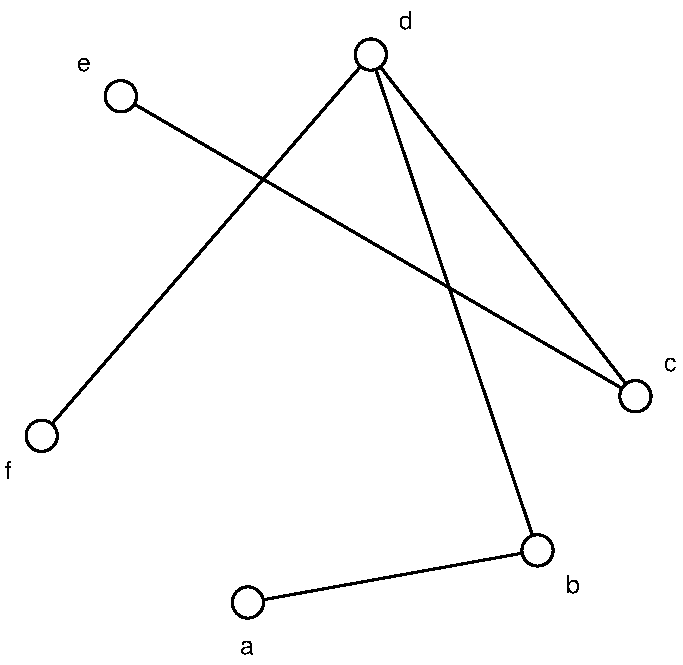
\includegraphics[width=\textwidth]{img/example_conflict_graph_segments.pdf}
          \caption{Line Segments}
  \end{subfigure}
  \hspace{2em}
  \VRule
  \hspace{2em}
  \begin{subfigure}[b]{0.4\textwidth}
          \centering
          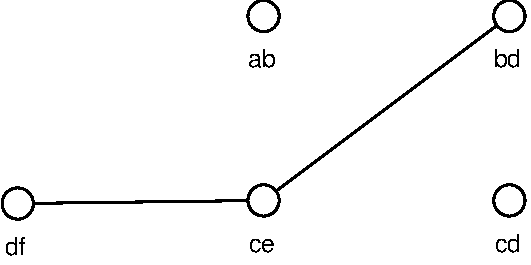
\includegraphics[width=\textwidth]{img/example_conflict_graph.pdf}
          \caption{Conflict Graph}
  \end{subfigure}  
  \caption{\label{fig:example_conflict_graph}Example of the Conflict %
    Graph for a given set of line segments %
    and the conflicts being all intersections}
\end{figure}

Now we can combine the previous definitions to characterize
triangulations. Note that we start off with a combinatorial
definition without any geometric components. In the course of this
chapter, we show how to apply this formulation to geometric problems.

\begin{definition}[Triangulation]
  Given the Complete Graph \(K_V = (V,E)\) for a vertex set \(V\)
  and a set of conflicts \(X\) for \(E\)
  such that the Conflict Graph \(\gls{Gconf}[(E,X)]\) is \gls{wcover}.
  A \emph{Triangulation} \(T(V,X) \subseteq E\) of \(V\) with respect
  to \(X\) is a maximum set of non-conflicting edges:
  \[
    e_i \in T(V,X)
    \iff e_i \in E
    \land \forall e_j \in T(V,X) : \{e_i,e_j\} \not\in X
  \]
\end{definition}

Bringing the Maximum Independent Set from \cref{sec:independent_set}
back to mind, we can see that a Triangulation is essentially the same
problem. Apart from Triangulations operating on the Conflict Graph,
both problems maximize the number of ``independent'' vertices.

\begin{theorem}[Equality of Triangulation and Maximum Independent Set]
  \label{thm:triangulation_independent_set}
  Every Triangulation \(T(V,X)\) of a vertex set \(V\) with respect
  to conflicts \(X\) is a Maximum Independent Set for the Conflict
  Graph \(\gls{Gconf}[(E,X)]\) and vice versa. Herein \(E\) are the
  edges of the Complete Graph \(K_V\).
  \begin{proof}
    \Cref{thm:triangulation_independent_set} follows directly from
    \cref{def:max_independent_set,thm:well_covered_independent_set}.
  \end{proof}
\end{theorem}

Now we can make use of \cref{alg:greedy_independent_set} from
\cref{cha:integer_programming} to gain a first bound on the time
complexity of finding \emph{any} Triangulation (for a given vertex
set and conflicts). Later, we give more accurate time bounds for
special classes of Triangulations.

\begin{theorem}[Time Complexity of Triangulations]
  \label{thm:time_complexity_triangulations}
  From
  \cref{%
    thm:triangulation_independent_set,%
    thm:well_covered_maximum_independent_set%
  }
  follows that finding a Triangulation \(T(V,X)\) of a vertex set
  \(V\) with respect to conflicts \(X\) takes \(O(|X|)\) time.
\end{theorem}

One important property of geometric objects has not been considered
for our definition of Triangulations yet: \emph{forbidden objects}.
Besides conflicting objects
from which only one can be part of the same Triangulation, there may
also be objects which are not wanted at all as we consider the
Complete Graph. This can be the case when a Triangulation is required
to lie completely within a certain boundary or when one object
overlaps multiple others.

\begin{definition}[Triangulation with Forbidden Edges]
  \label{def:triangulation_forbidden_edges}
  A \emph{Triangulation with Forbidden Edges} \(T(V,X,F)\) is a 
  Triangulation of the vertex set \(V\) with respect to conflicts
  \(X\) which does not contain any of the edges in \(F\):
  \[ \forall e \in F : e \not\in T(V,X,F) \]
\end{definition}

Even though \cref{def:triangulation_forbidden_edges} models
geometric triangulation problems better, it is not solvable in
polynomial time anymore (assuming P\(\not=\)NP). Many geometric
triangulations are solvable in polynomial time however (as we see
later) so this approach is clearly not the best one to solve them.

\begin{theorem}[NP-completeness of Triangulation with Forbidden Edges]
  The decision problem whether 
  a Triangulation with Forbidden Edges \(T(V,X,F)\) exists
  is NP-complete.
  \cite[triangulation existence problem]{triangulation_forbidden_edges}
\end{theorem}

There is another approach to ensure that boundary is part of a
Triangulation which we call \emph{constraints}. Basically, we require
a Triangulation to contain certain objects, e.g. the boundary. This
leaves the problem that objects outside the boundary can be part of
the Triangulation, but those can be removed from the Triangulation
in polynomial time (because triangulations have polynomial size).

\begin{definition}[Constrained Triangulation]
  \label{def:constrained_triangulation}
  A \emph{Constrained Triangulation} \(T(V,X,C)\) is a Triangulation
  of the vertex set \(V\) with respect to conflicts \(X\) which 
  contains the edge constrains \(C\):
  \[ \forall e \in C : e \in T(V,X,C) \]
\end{definition}

In contrast to the Triangulation with Forbidden Edges, Constrained
Triangulations can be found in polynomial time. Therefore we slightly
modify \cref{alg:greedy_independent_set} to begin with the constraints
as initial Independent Set and then proceed as before. This assumes
that the constraints themselves are all valid and not conflicting.
Even without that guarantee, an additional check before running the
algorithm would require at most quadratic time with respect to the
constraints---so the whole running time is still polynomial.

\begin{theorem}[Time Complexity of Constrained Triangulations]
  Using \cref{alg:greedy_independent_set}
  a Constrained Triangulation \(T(V,X,C)\) of the vertex set \(V\)
  with respect to conflicts \(X\) and constrains \(C\)
  can be calculated in \(O(|C|^2 + |X|)\) time.
  In case \(C\) is guaranteed to have the Independent Set property,
  running time reduces to \(O(|X|)\).
\end{theorem}

\section{Point Set Triangulations}
\label{sec:point_set_triangulations}
In this \namecref{sec:point_set_triangulations} we present the first
geometric triangulation problem and draw the connection to our
previous definition. The difference between a (topological)
Triangulation as we have defined it earlier and a Point Set
Triangulation which we get to in this
\namecref{sec:point_set_triangulations} can be seen as the distinction
between a graph and its embedding.

To make things clear, we start by defining some geometric terms which
we use in the following. The equivalent of edges in a topological
triangulation are line segments for a geometric triangulation in the
plane. Since line segments are not restricted to the plane, we do not
focus on two dimensions here. However according to some definitions,
triangulations for higher dimensions contain also geometric objects
of higher dimension (e.g. tetrahedra in three dimensions). For
simplicity, we consider those objects be implicitly defined by their
bounding line segments.

\begin{definition}[Line Segments]
  A \emph{line segment} \(s=(p,q)\) is determined by its endpoints
  \(p,q\in P\) with \(P\) being a point set (of arbitrary dimension). 
  For compatibility with other definitions,
  \(s\) is directed from \(p\) to \(q\), i.e. \((p,q)\not=(q,p)\)
  and contains all points \(m\) ``between'' \(p\) and \(q\):
  \[ m \in s \iff \exists a\in [0,1] : m = p + a \cdot (q-p) \]
\end{definition}

Clearly, the counterpart of conflicting edges are intersecting line
segments. Nevertheless, depending on the definition, intersection of
two line segments with the same endpoint is either empty or the common endpoint.
This is why we assume intersection of any geometric objects to be the
set intersection of all (usually infinitely many) points contained in
the objects and introduce the already widely used term \gls{cross}:

\begin{definition}[Crossing]\label{def:crossing}
  Two line segments \(s_i=(p_i,q_i)\) and \(s_j=(p_j,q_j)\) with 
  different slope are \gls{cross}, if their intersection is not empty
  and not an endpoint, i.e.
  \[
    s_i, s_j~\gls{cross}
    \iff
    (p = s_i\cap s_j) \land
    (|s_i\cap s_j| = 1) \land
    (p \not\in \{p_i,q_i,p_j,q_j\})
  \]

  Two line segments \(s_i\) and \(s_j\) are \gls{ncross}
  if they are not \gls{cross}.
  A set \(S\) of line segments is \gls{cross}
  if at least two segments \(s_i, s_j \in S\) are \gls{cross}.
  It is \gls{ncross} if each pair \(s_i, s_j \in S\) is \gls{ncross}.
\end{definition}

We do not require points to be in general position which is why we
have to deal with degeneracies in the following. General position
often preempts interesting instances---e.g. those which are heavily
symmetric. Additionally, many man-made structures aim for
collinearity, so extra effort has to be expended to make real world
instances fit the general position requirements. The following
\namecref{def:overlapping_segments} identifies all unwanted line
segments in case of collinear points. Refer to
\cref{fig:overlapping_segments} for examples of such degeneracies.

\begin{definition}[Overlapping Line Segments]
  \label{def:overlapping_segments}
  Given a point set \(P\) and a line segment \(s = (p,q)\) with
  \(p,q \in P\). \(s\) is \gls{overlap} in \(P\) if and only if
  there is a point \(p' \in P\) which lies in its interior:
  \[
    s~\gls{overlap}
    \iff  \exists p' \in P : (p' \in s) \land (p' \not\in \{p,q\})
  \]
  \(s\) is \gls{noverlap} if it is not \gls{overlap}.
\end{definition}

\begin{figure}[ht]
  \centering
  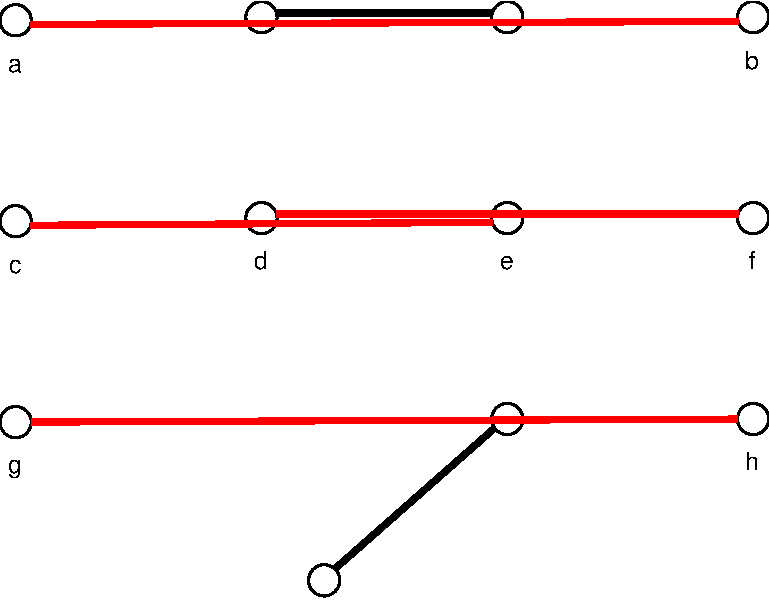
\includegraphics[width=0.5\textwidth]{img/example_overlapping.pdf}
  \caption{\label{fig:overlapping_segments}%
    Examples of overlapping line segments %
    (\(\{a,b\}, \{c,e\}, \{d,f\}, \{g,h\}\))%
  }
\end{figure}

Earlier in this \namecref{sec:point_set_triangulations}, we already
mentioned the connection between topological and geometric
triangulations---and here comes the formal definition. Note that
we distinguish between points (which have a geometry, i.e.
coordinates) and vertices (which are solely topological objects).

\begin{definition}[Topological Representation]
  A vertex set \(V(P)\) \emph{represents} a point set \(P\) if there
  is exactly one vertex \(v_p \in V(P)\) for each point \(p \in P\)
  and \(v_p\) can be identified by \(p\) and vice versa.
\end{definition}

After having all basic terms at hand, we now proceed with
\emph{Point Set Triangulations}. They are the geometric equivalent
of topological triangulations for point sets. To emphasize that
Point Set Triangulations without further restrictions can be 
calculated in polynomial time (compare
\cref{thm:time_complexity_triangulations,%
  thm:time_complexity_planar_point_set_triangulations}),
we avoid a definition based on Triangulations with Forbidden Edges (see
\cref{def:triangulation_forbidden_edges})---despite the fact that
overlapping line segments are forbidden edges. Note that in this case that
finding a Triangulation involving overlapping line segments takes
polynomial time. Afterwards they can be replaced by the line segments
that they include in polynomial time (because there are polynomially
many line segments).

\begin{definition}[Point Set Triangulation]
  \label{def:point_set_triangulation}
  The Triangulation \(T(P)\) of a point set \(P\)
  is a triangulation \(T(P) = T(V,X)\)
  where the vertex set \(V=V(P)\) represents \(P\), 
  the conflicts \(X\) are all \gls{cross} line segments, 
  and which contains no \gls{overlap} line segments:
  \begin{alignat*}{1}
    (p,q), (p',q')~\gls{cross}
    &\iff \left\{ \{v_p,v_q\}, \{v_{p'},v_{q'}\} \right\} \in X \\
     (p,q)~\gls{overlap}
    &\implies \{v_p,v_q\} \not\in T(P)
  \end{alignat*}

  For convenience we define \(s=(p,q) \equiv e=\{v_p,v_q\}\) such
  that \(s \in T(P) \iff e \in T(P)\). See also
  \cite[Section 9.1]{deberg_compgeom} for a slightly different yet
  equivalent definition of Point Set Triangulations.
\end{definition}

The asymptotic time complexity of finding a Triangulation can be 
improved for the special case of Point Set Triangulations. For example
by making use of sweep line algorithms which exploit that
Triangulation properties can be ensured locally, the running time
drops to \(O(n \log n)\) as in \cite{fortunes_algorithm}.

\begin{theorem}[Time Complexity of Planar Point Set Triangulation]
  \label{thm:time_complexity_planar_point_set_triangulations}
  A planar point set \(P \subseteq \gls{R}[^2]\) can be triangulated
  in \(O(n \log n)\) time with \(n = |P|\).
  \cite[Theorem 9.12]{deberg_compgeom}
\end{theorem}

In \cref{def:constrained_triangulation} we already showed a way to
force certain objects (e.g. boundaries) to be part of a Triangulation.
The same concept can be transferred to Point Set Triangulations as in
the following \namecref{def:constrained_point_set_triangulation}:

\begin{definition}[Constrained Point Set Triangulation]
  \label{def:constrained_point_set_triangulation}
  A \emph{Constrained Point Set Triangulation} \(T(P,C)\)
  of a point set \(P\) with line segment constraints \(C\)
  is a Point Set Triangulation \(T(P,C) = T(P)\)
  such that \(C \subseteq T(P, C)\).
\end{definition}

The same time bound holds in the presence of constraints. Sweep line 
algorithms can be modified for taking constraints into account. Note
that constraints can destroy desired properties of a Point Set
Triangulation (such as large inner angles). We come back to some of
those additional requirements later in this
\namecref{cha:triangulations}.

\begin{theorem}[Constrained Point Set Triangulation]
  A \emph{Constrained Point Set Triangulation} \(T(P, C)\)
  for a planar point set \(P \subseteq \gls{R}^2\)
  and line segment constraints \(C \subseteq P^2\)
  can be calculated in \(O(n \log n)\) time.
  \cite{constrained_triangulation}
\end{theorem}

\section{Intersection Graph}
\label{sec:intersection_graph}
When we defined the Point Set Triangulation
(\cref{def:point_set_triangulation}), we assumed that the set of 
conflicts (i.e. all pairs of \gls{cross} line segments) is already
given, which might not be they case. This
\namecref{sec:intersection_graph} fills the gap by introducing the
\emph{Intersection Graph}. For consistency with other definitions, we
kept the name even though it actually contains only \gls{cross} line
segments (according to our previous definition of intersection).

\begin{definition}[Intersection Graph]
  \label{def:intersection_graph}
  For a set of line segments \(S\) the
  \emph{Intersection Graph} \(\gls{Gcross}[(S)] = (V_S,X)\) consists
  of a vertex \(v_s \in V_S\) for every line segment \(s \in S\)
  and an edge \(\{v_{s_i}, v_{s_j}\} \in X\)
  for every pair of \gls{cross} segments \(s_i, s_j \in S\).
  It is the geometric equivalent of the Conflict Graph
  (see \cref{def:conflict_graph}).
\end{definition}

Generating the Intersection Graph for line segments in the plane can
be done efficiently using an output sensitive sweep line algorithm.
By output sensitive we refer to the (asymptotic) running time
depending on the output size, i.e. how many line segments intersect.

\begin{theorem}[Time Complexity of Intersection Graph]
  \label{thm:sweep_bound}
  Given a set of line segments \(S\) in the plane,
  the Intersection Graph \(\gls{Gcross}[(S)] = (V_S,X)\)
  can be calculated in \(O(m \log m + i \log m)\) time
  where \(m = |V_S| = |S|\)
  and \(i = |X|\) is the number of intersections in \(S\).
  \cite[Lemma 2.3]{deberg_compgeom}
\end{theorem}

The referenced method works well for a small number of
intersections but fails to do so when there are significantly more
intersections than line segments. Let us first state how many
intersections there are when all possible connections in a point set
are considered:

\begin{theorem}[Complexity of Point Set Intersections]
  \label{thm:point_set_intersections}
  For a planar point set \(P\) with \(n\) points,
  the set of all line segments \(S\) with endpoints in \(P\)
  has \(\Theta(n^4)\) intersection points.~\cite{quadrilaterals_bound}
  Thus calculating the Intersection Graph for \(S\)
  takes \(\Omega(n^4)\) time.
\end{theorem}

This bound on the number of intersections shows that the sweep line
approach is not a good choice in our case---especially because it does
not reach the lower time bound of \(\Omega(n^4)\) (even though we have
not yet shown that this is possible at all).

\begin{theorem}[Non-Optimality of Sweep Algorithm for Point Sets]
  The sweep algorithm presented in \cite[Section 2.1]{deberg_compgeom}
  with the time complexity of \cref{thm:sweep_bound}
  is not optimal for finding
  all \gls{cross} line segments with endpoints in a given
  planar point set \(P\) of size \(n=|P|\)
  as it takes \(O(n^4 \log n)\) time.
\end{theorem}

Now let us consider the straightforward approach of simply checking
all pairs of line segments if they are \gls{cross}. 
\Cref{alg:naive_intersection} realizes this idea with a small
optimization: To avoid checking each pair of line segments twice, we
take the length \(|s|\) of a line segment \(s\) into account. The same
can be done by using a sorted list instead of a set for the line
segments (which even works for line segments with the same length).

\begin{algorithm}
  \DontPrintSemicolon
  
  \KwIn{Set of line segments \(S\)}
  \KwOut{Intersection Graph \(\gls{Gcross}[(S)] = (V_S,X)\)}
  
  Set \(V_S = \{v_s : s \in S\} \) \;
  Set \(X = \emptyset\) \;
  \ForEach{\(s \in S\)}{
    \ForEach{\(\gls{scross} \in S\) with \(|s| \leq |\gls{scross}|\)}{
      \If{\(s\) and \gls{scross} are \gls{cross}}{
        Add \(\{v_s, v_{\gls{scross}}\}\) to \(X\) \;
      }
    }
  }
  \KwRet{\(\gls{Gcross}[(S)] = (V_S,X)\)}
  \caption{\label{alg:naive_intersection}Naive Intersection Algorithm}
\end{algorithm}

We can directly deduce the asymptotic running time from the algorithm
and its correctness is implied by the fact that every possible
combination of potentially \gls{cross} line segments is considered.

\begin{theorem}[Time Complexity and Correctness of \Cref{alg:naive_intersection}]
  \Cref{alg:naive_intersection} finds all \gls{cross} line segments
  in \(O(m^2)\) time with \(m = |S|\).  
\end{theorem}

Again, the most simple approach is indeed asymptotically optimal for
our application as for \cref{alg:greedy_independent_set} in
\cref{cha:integer_programming}. Additionally
\cref{alg:naive_intersection} does not assume that the set of line
segments is planar.

\begin{theorem}[Optimality of \Cref{alg:naive_intersection} for Point Set]
  \Cref{alg:naive_intersection} is asymptotically optimal
  for finding all \gls{cross} line segments
  with endpoints in a given planar point set \(P\)
  as it takes \(O(n^4)\) time for \(n = |P|\).
\end{theorem}

\section{Polygon Triangulations}
One case where boundary needs to be taken into account is when
triangulating the interior of a polygon. We can reduce this case to
the already defined Constrained Point Set Triangulation of the
previous \cref{sec:point_set_triangulations}:

\begin{definition}[Polygon Triangulation]
  A Triangulation \(T(P)\) of a polygon \(P\) bounded by line segments
  are all boundary and interior edges of \(P\)
  in a Constrained Point Set Triangulation of the polygon vertices
  with the polygon boundary as constraints.
\end{definition}

We can also reverse the reduction such that a Point Set Triangulation
can be constructed by finding a Polygon Triangulation first:

\begin{theorem}[Generalization of Point Set Triangulation]
  Every triangulation of a point set \(P\)
  is a triangulation \(T(\conv(P) \cup P)\)
  of the polygon bounded by the convex hull \(\conv(P)\) of \(P\)
  and containing all inner points of \(P\).
  \begin{proof}
  First recall that the Triangulation \(T(\conv(P) \cup P)\)
  is a Constrained Point Set Triangulation \(T_c(P,C)\) for the point
  set \(P\) with the constraints \(C = \conv(P)\) being all line
  segments on the convex hull of \(P\). Now we only need to show that
  the choice of \(C\) does not exclude any Point Set Triangulation by
  proving that every line segment \(s \in C\) has to be part of every
  Point Set Triangulation for \(P\):
  
  Assume that there is a Point Set Triangulation \(T'\) for \(P\)
  which does not contain a line segment \(s \in C\). Because \(T'\)
  is a maximal set of \gls{ncross} line segments by definition,
  there has to be a line segment \(s' \in T'\) such that \(s\) and
  \(s'\) are \gls{cross}. This implies that the endpoints of \(s'\)
  have to be on opposite sides of \(s\) and since \(s\) is part of
  the convex hull, one of the endpoints of \(s'\) has to lie outside
  of the convex hull. This contradicts the definition of the convex
  hull.
  \end{proof}
\end{theorem}

\section{Edge Flipping}
Besides the already mentioned sweep algorithms for Triangulations of
planar point sets, there is another common approach called
\emph{Edge Flipping}, which starts with any Triangulation and 
iteratively replaces an edge by another one until the Triangulation 
has a certain desired property (e.g. large inner angles).

\begin{definition}[Edge Flip]
  \label{def:edge_flip}
  Given a triangulation \(T(V,X)\) for a vertex set \(V\) with respect
  to a set of conflicts \(X\), \((e, f)\) with \(e \in T(V,X)\) and
  \(f \not\in T(V,X)\) is an \emph{edge flip} iff
  \(T(V,X) \setminus \{e\} \cup \{f\}\) is a triangulation for \(V\)
  with respect to \(X\).
\end{definition}

An edge flip is not possible with any pair of edges. For planar point
sets, both edges need to be diagonals of a convex quadrangle. More
generally, they can only be conflicting edges:

\begin{theorem}[Edge Flips are Conflicts]
  Given a Triangulation \(T(V,X)\) for a vertex set \(V\)
  with respect to a set of conflicts \(X\),
  every edge flip \((e,f)\) is a conflict: \(\{e,f\} \in X\).
  \begin{proof}
  Assume \(\{e,f\} \not\in X\). Further assume that
  \[ \lnot\exists e' \in T(V,X)\setminus\{e\}: \{e', f\} \in X. \]
  Then \(f\) can be added to \(T(V,X)\) (without removing \(e\)) and
  therefore \(T(V,X)\) is no triangulation---which is a 
  contradiction. Now let \(e' \in T(V,X)\setminus\{e\}\) such that
  \(\{e', f\} \in X\). Then \(e' \in T(V,X)\setminus\{e\} \cup f\)
  ---which contradicts that \(T(V,X)\setminus\{e\} \cup f\) is a
  triangulation. Therefore every edge flip \((e,f)\) is a conflict.
  \end{proof}
\end{theorem}

Continuously applying edge flips to a Triangulation can be seen as
traversing a path within the graph of all Triangulations. Such a graph
with vertices for every Triangulation and edges for every possible
edge flip is called the \emph{Flip Graph}. An example can be seen in
\cref{fig:example_flip_graph}.

\begin{definition}[Flip Graph]
  \label{def:flip_graph}
  The \emph{Flip Graph} \(\gls{Gflip}[(V,X)] = (V_T,\gls{Eflip})\)
  for a vertex set \(V\) and edge conflicts \(X\)
  contains a vertex \(v \in V_T\) for every triangulation of \(V\)
  with respect to \(X\) and edges \(e \in \gls{Eflip}\)
  for every possible edge flip.
\end{definition}

\begin{figure}[ht]
  \centering
  \begin{subfigure}{0.3\textwidth}
    \centering
    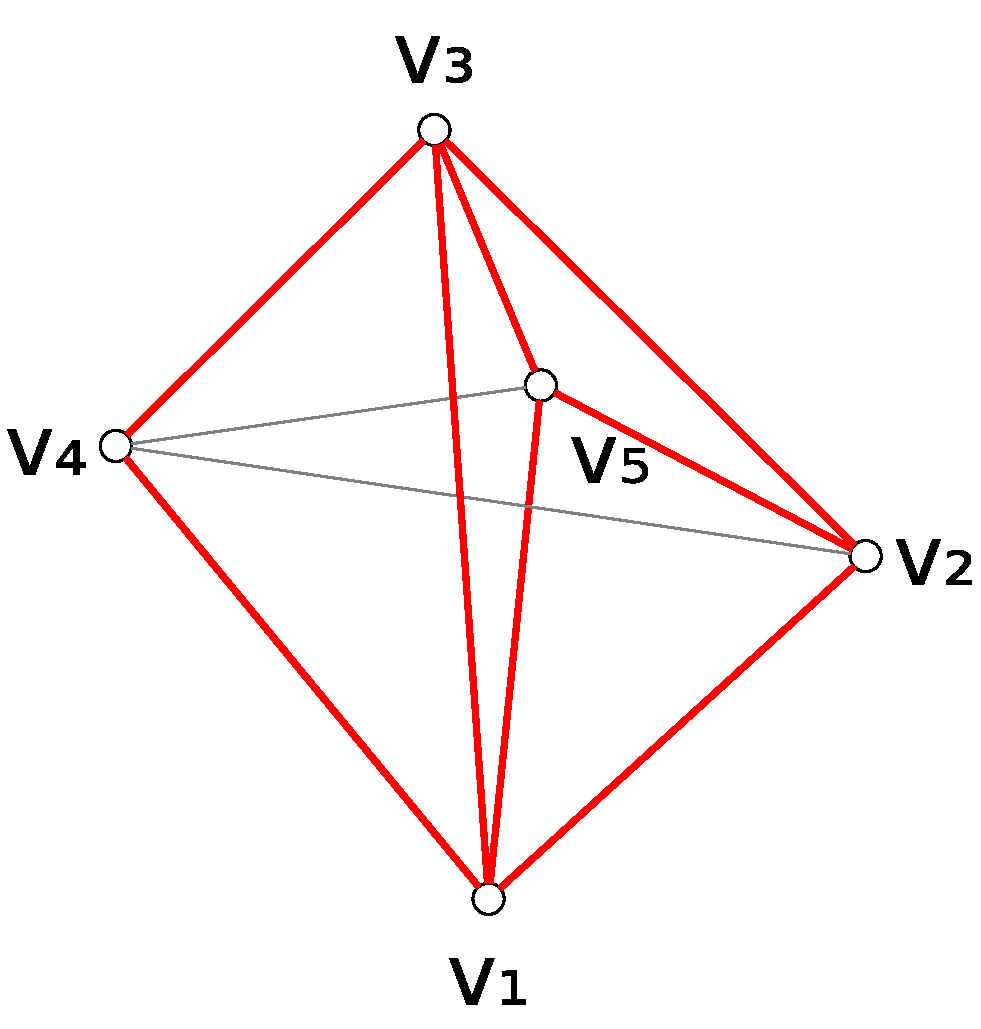
\includegraphics[width=\textwidth]{img/example_triangulation_1.pdf}
    \caption{}
  \end{subfigure}
  \hspace{0em}
  \VRule
  \hspace{0em}
  \begin{subfigure}{0.3\textwidth}
    \centering
    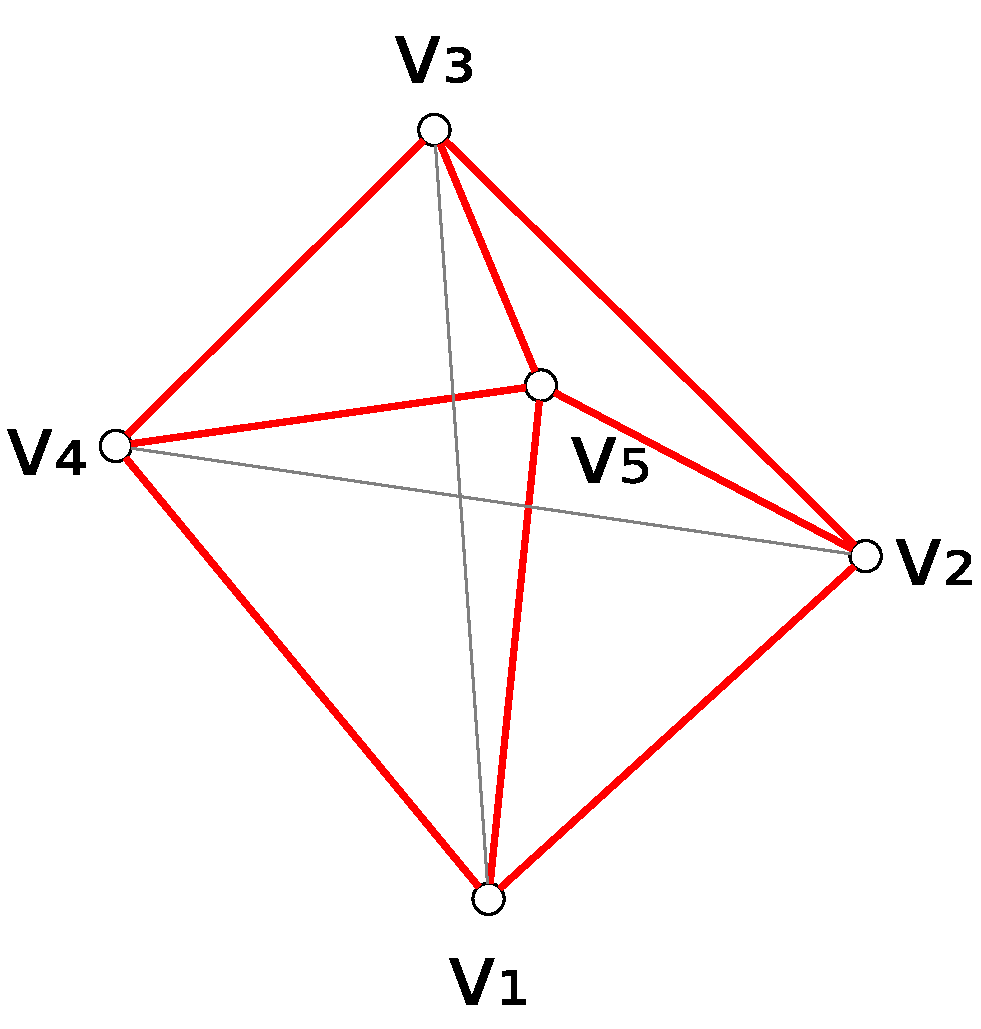
\includegraphics[width=\textwidth]{img/example_triangulation_2.pdf}
    \caption{}
  \end{subfigure}
  \hspace{0em}
  \VRule
  \hspace{0em}
  \begin{subfigure}{0.3\textwidth}
    \centering
    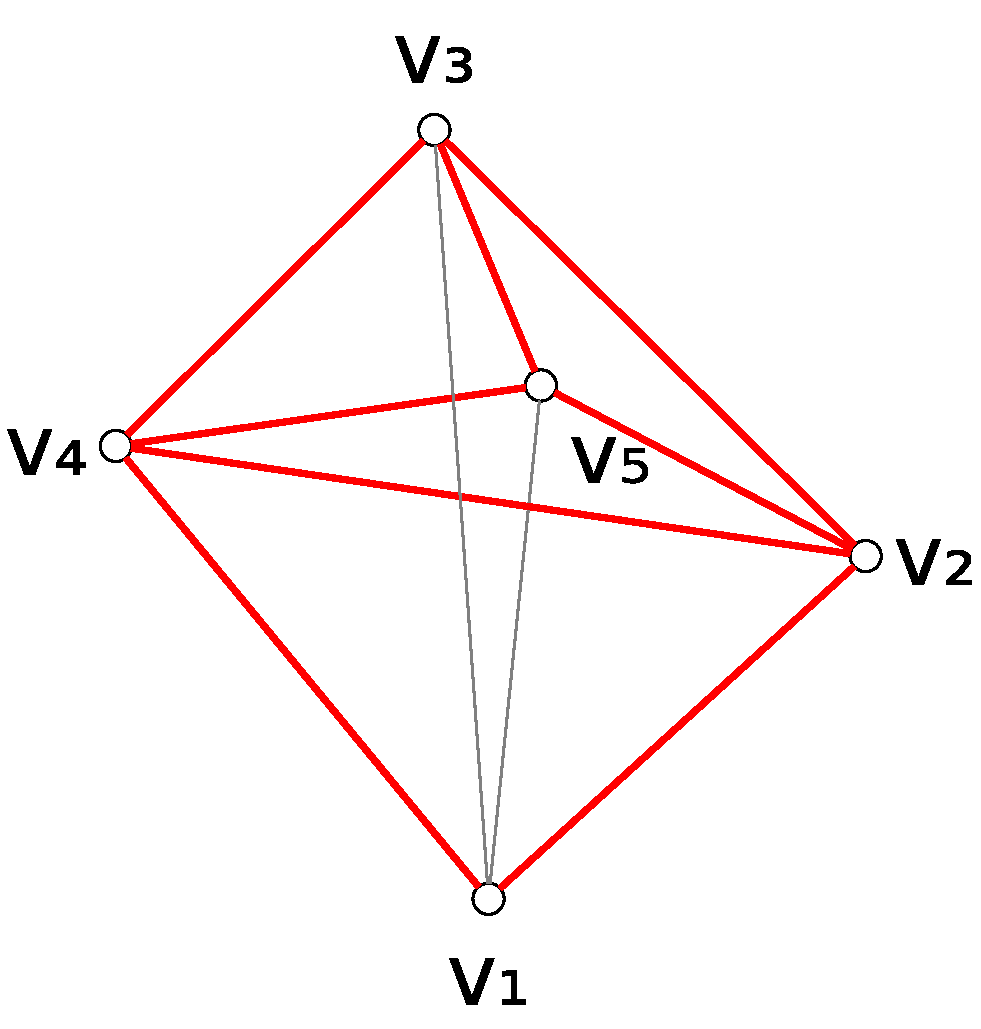
\includegraphics[width=\textwidth]{img/example_triangulation_3.pdf}
    \caption{}
  \end{subfigure}
  
  \vspace{2em}
  \begin{subfigure}{0.7\textwidth}
    \centering
    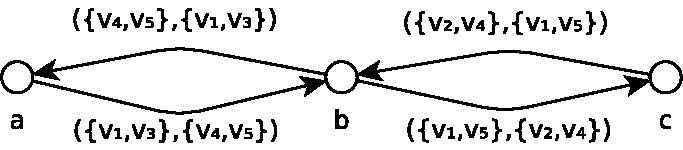
\includegraphics[width=\textwidth]{img/example_flip_graph.pdf}
    \caption{Flip Graph}
  \end{subfigure}
  \caption{\label{fig:example_flip_graph}%
    Example triangulations and their flip graph}
\end{figure}

Changing any Triangulation into any other Triangulation using edge
flips is only possible if the Flip Graph is connected; i.e. there is
a path between every two vertices. This is the case for two dimensions
but is not yet completely explored for higher dimensions.

\begin{theorem}[Connectivity of the Flip Graph]
  The Flip Graph \(\gls{Gflip}[(V,X)]\) is connected in two dimensions
  \cite[Behauptung 4]{flip_graph_connected} and has a diameter of
  at most \(6n - 30\) for \(n = |V|\).~\cite{flip_graph_diameter}
  Therefore every Triangulation \(T(V,X)\) of a vertex set \(V\)
  with respect to edge conflicts \(X\) can be transformed into any
  other Triangulation of \(V\) with respect to \(X\) in \(O(n)\)
  time.
  
  For three dimensions, it is still an open problem whether
  or not the Flip Graph is connected.~\cite{flip_graph_3d}
\end{theorem}

Another issue of edge flipping algorithms are Triangulations
which have additional non-locally restricted objectives. If for every
two edges in a potential edge flip it can be determined which one
improves the Triangulation with respect to the objective, the Flip
Graph can be searched for a Triangulation for which all edge flips
would worsen the solution with respect to the objective. This is
possible for optimizing the inner angles of triangles. In
\cref{cha:mmlt} we show that it is not possible for the \gls{MMLT}.
Therefore the whole Flip Graph has to be considered, which has
exponential size.

\section{Related Work}
\label{sec:related_work}
In the following, we briefly mention some results for different kinds
of Triangulations. These problems have kept researchers busy
for over 100 years~\cite{triangulation_hilbert} and several
books have been written which cover the topic,
e.g.~\cite{triangulation_book}.

The most famous kind is probably the Delaunay Triangulation
\cite[Section 9.2]{deberg_compgeom}. It forces every circumcircle
of a triangle to be empty of other points and therefore maximizes
the minimum angle \cite[Theorem 9.9]{deberg_compgeom}. There is an
edge flipping algorithm which calculates it in \(O(n \log n)\) 
expected time using \(O(n)\) space 
\cite[Theorem 9.12]{deberg_compgeom}.

The counterpart of a Delaunay Triangulation, 
minimizing the maximum angle, takes \(O(n^2 \log n)\) time and
\(O(n)\) space~\cite{triangulation_edge_insertion}. The same
approach can also produce triangulations which maximize the minimum 
height of a triangle. Finally, the same reference shows also that 
minimizing the maximum slope and minimizing the maximum eccentricity 
can both be done in \(O(n^3)\) time and \(O(n^2)\) space.

Optimizing the area of triangles has been studied
in~\cite{triangulation_area} resulting in \(O(n^2 \log n)\) time
and \(O(n^2)\) space for minimizing or maximizing the area.

There are several results for optimal edge length Triangulations.
One of the first publications \cite{triangulation_minmax_length}
shows that minimizing the maximum edge length can be done in
\(O(n^2)\) time. Minimizing the edge length sum (also known as the 
Minimum Weight Triangulation) was proven NP-hard \cite{mwt_complexity}.
Maximizing the minimum edge length was stated as an open problem~%
\cite{triangulation_minmax_length} but 20 years later it has been
shown that it is NP-complete~\cite{mmlt_complexity}. It remains NP-hard
for polygons with holes and interior points \cite{mmlt_polygons}
but can be solved in \(O(n^3)\) time for simple
polygons and even in linear time for convex polygons
\cite{mmlt_convex_polygons}.

%---------------------------------------------------------------------##########
